\documentclass[11pt, letterpaper]{article}

% PACKAGES
\usepackage{graphicx}
\usepackage{caption}
\usepackage{multirow}
\usepackage{makecell} % for more vertical space in cells
\setcellgapes{5pt}
\usepackage{amsmath}
\usepackage{amsfonts}
\usepackage{subcaption}%
\usepackage{amssymb}
\usepackage{amsthm}
\usepackage{mathtools}
\usepackage{verbatim}
\usepackage{matlab-prettifier}
\usepackage{pgfplots}
\usepackage{hyperref}
\usepackage[
    backend=biber,
    style=numeric,
    ]{biblatex}
\addbibresource{sources.bib}

% PAGE SETUP
\setlength{\textheight}{9in}
\setlength{\topmargin}{-0.75in}
\setlength{\headheight}{15pt}
\setlength{\textwidth}{7in}
\setlength{\oddsidemargin}{-0.2in}
\setlength{\parskip}{6pt}
\setlength{\parindent}{0pt}
% \renewcommand{\headrulewidth}{1pt}
\setlength{\headsep}{1cm}

% OPERATORS
\DeclareMathOperator{\R}{\mathbb{R}}

% THEOREMS
\newtheoremstyle{perchance}{10pt}{10pt}{}{}{\bfseries}{}{.5em}{}
\theoremstyle{perchance}
\newtheorem{innercustomthm}{Theorem}
\newenvironment{customthm}[1]{\renewcommand\theinnercustomthm{#1}\innercustomthm}{\endinnercustomthm}
\newtheorem*{definition}{Definition}
\newtheorem*{theorem}{Theorem}

% DOC INFO
\title{\vspace{-1.25cm}An Introduction to Spectral Clustering\vspace{-0.5cm}}
\author{Andre Gormann 301332332 \\Eunice Javier 301344291\vspace{-0.25cm}}
\date{December 2023}

\begin{document}

    \vspace{-10mm}

\maketitle
    
    \vspace{-15mm}
    
\section{Introduction}\label{sec:intro}

    In graph theory, there are situations where meaning must be extracted from the edge connections between nodes. One method of achieving this is something called clustering. Generally speaking, clustering is a way of grouping things that are similar and separating things that are dissimilar \cite{wikicluster}. While we are motivated to cluster graphs, there is another relevant form of clustering: data clustering. As the name suggests, it is concerned with the grouping of data. \emph{Spectral} clustering, in a nutshell, is a novel way of turning a graph clustering problem into a data clustering problem by utilizing the spectrum of matrices extracted from a graph.
    
    What these terms mean will be properly explained in Section \ref{sec:prelim}, along with some important facts from graph theory and linear algebra. We will detail the ideas behind spectral clustering in Section \ref{sec:spec}, along with two algorithms in Section \ref{sec:algo}. Section \ref{sec:valid} will detail the identification of good clusters and bad ones, along with experimental results in Section \ref{sec:exp}. Section \ref{sec:conc} will include closing remarks as well as further areas for experimentation and analysis. All of the code written can be found in \ref{sec:code}.
    
\section{Preliminaries}\label{sec:prelim}

    \subsection{Graph Theory and Linear Algebra}
    
        \begin{definition}
            A \emph{graph} is a set $G = \{V, E\}$, where $V$ is a set of vertices (or nodes), and $E$ is a set of unordered vertices, whose elements are called edges. If there exists a finite sequence of edges in $G$ such that every vertex is traversed, then we say $G$ is \emph{connected}. Otherwise, it is disconnected. 
        \end{definition}
    
        \vspace{-3mm}
        
        Technically speaking, what we have defined is an \emph{undirected and unweighted graph}. For the sake of brevity, we will use this definition when referring to any graphs moving forward. Secondly, due to the properties of connected graphs, all graphs can be assumed to be connected unless stated otherwise.
        
        Now, given any graph $G$, we can construct three fundamental matrices:
        
        \begin{definition}
            The \emph{adjacency} matrix of graph $G$ is a symmetric matrix $A \in \R^{n \times n}$ such the entry $a_{ij}$ is 1 if ${i, j} \in E$, and 0 otherwise. The \emph{degree} matrix is a diagonal matrix $D \in \R^{n \times n}$ such that $d_{ii}$ is the sum of row $i$ of $A$. The \emph{Laplacian} matrix $L$ is defined to be $L = D - A$.
        \end{definition}
        
        \vspace{-3mm}
    
        To better illustrate this, consider a graph $G$ defined by 
        \[V = \{1, 2, 3, 4\} \,\text{ and }\, E = \{\{1, 2\}, \{1, 3\}, \{3, 4\}\}.\] 
        Then we have
        \[A = 
        \begin{bmatrix}
        0 & 1 & 1 & 0 \\
        1 & 0 & 0 & 0 \\
        1 & 0 & 0 & 1 \\
        0 & 0 & 1 & 0 \\
        \end{bmatrix}, \qquad D = \begin{bmatrix}
        2 & 0 & 0 & 0 \\
        0 & 1 & 0 & 0 \\
        0 & 0 & 2 & 0 \\
        0 & 0 & 0 & 1 \\
        \end{bmatrix}, \qquad L = \begin{bmatrix}
        \phantom{-}2 & -1 & -1 & \phantom{-}0 \\
        -1 & \phantom{-}1 & \phantom{-}0 & \phantom{-}0 \\
        -1 & \phantom{-}0 & \phantom{-}2 & -1 \\
        \phantom{-}0 & \phantom{-}0 & -1 & \phantom{-}1 \\
        \end{bmatrix}. \]
    
        \begin{definition}
            For a matrix $A \in \R^{m \times n}$, an \emph{eigenvector} is a vector $x \in \R^{n}$ that satisfies the following relation: $Ax = \lambda x$, where $\lambda \in \R$. That is to say that the image of $x$ under $A$ is a scalar multiple of $x$. The magnitude of this scaling, $\lambda$, is known as the \emph{eigenvalue} associated with the eigenvector $x$.
        \end{definition}
        
        \vspace{-3mm}
        
        The Laplacian matrix is fundamental to spectral clustering for several reasons. One of them being the properties listed below.
        
        \begin{theorem}
            The Laplacian matrix $L$ of a graph $G$ is
            \begin{enumerate}
                \item[(i)] symmetric;
                \item[(ii)] singular;
                \item[(iii)] positive semi-definite.
            \end{enumerate}
        \end{theorem}
    
        \vspace{-3mm}
    
        Since $L$ is defined to be the difference between two symmetric matrices (diagonal matrices are symmetric), it is trivially symmetric. It is also easy to see that by construction, the vector $x = [1 \, \ldots \, 1]^T \in \R^n$ is a solution to the eigenvalue problem; namely, $Lx = 0$. Thus, it follows that the Laplacian is singular \parencite[\S 22.1]{bennett}. The proof for positive semi-definiteness is fairly involved and will not presented.
    
        By virtue of $L$ being symmetric, we are guaranteed that all eigenvalues are real-valued. Further, by $L$ being positive semi-definite, we can apply a well-order to the spectrum (the set of eigenvalues) whose importance will be seen in Section \ref{sec:spec}. Traditionally, the focus is often on the largest eigenvalues of a matrix. In spectral clustering, we are concerned with the \emph{smallest} eigenvalues. Of these eigenvalues, there is one so important that it gets its own name.

    \subsection{Fiedler Value and Vector}
    
        \begin{definition}
            The \emph{Fiedler value} or \emph{algebraic connectivity} \cite{bennett, wikialgcon} of a graph $G$ is defined as the second smallest eigenvalue, $\lambda_1$, of its graph Laplacian, $L$. The \emph{Fiedler vector} is the eigenvector $x_1$ such that $Lx_1 = \lambda_1x_1$.
        \end{definition}
    
        \vspace{-3.5mm}    
        
        We have already seen that the Laplacian is singular and positive semi-definite, and so the smallest eigenvalue must be 0. If the graph $G$ is connected, then the Fiedler value will be non-zero. Otherwise, it is zero. Accordingly, when the Fiedler value is non-zero, it can be a good indicator of how connected the graph is; values closer to zero indicate poor connectivity, and values significantly greater than 1 indicate strong connectivity. Hence, the Fiedler value can also be referred to as the algebraic connectivity of the graph.
    
        The Fiedler vector $x_1$ can be thought of as a one-dimensional representation of the structure of graph $G$, whose components signify relations between regions of the graph by way of how close they are numerically.
    
        Returning to the previous example, we have that $\lambda_1 = 0.5858$ which signifies some level of connectivity. The corresponding eigenvector is
        \[x_1 = \begin{bmatrix}
            0.2706 & 0.6533 & -0.2706 & -0.6533
        \end{bmatrix}^T\]
        The first entry is relatively close to the second and third entry, while quite far from the fourth. Examining the graph structure, we observe an edge connection between vertex 1 to vertices 2 and 3, while there is none present between vertex 1 and 4. As the number of vertices and edges increases, this behavior has been observed to continue.
    
        In graph clustering, one might consider doing so based on the sign or the distances between these components. Both of these ideas will be further explored in Sections \ref{sec:spec} and \ref{sec:algo}.

\section{Spectral Clustering}\label{sec:spec}

    As stated prior, the eigenvalues and eigenvectors of the graph Laplacian are the primary concern of spectral clustering. In practice, how these are utilized is subjective and context-dependent. In this paper, we show no regard for the eigenvalues and instead focus all of our attention on the eigenvectors. The reason for this is that we are considering a specific subset of graphs: those that are connected. Because of this choice, we are guaranteed that the Fiedler value is non-zero (and hence so is every other eigenvalue except $\lambda_1$ by the well-ordering of the spectrum).

    We utilize these eigenvectors by viewing them as column vectors and concatenating them horizontally into a matrix $X$ \cite{wikispec}:
    \[X = \left[\begin{array}{c | c | c | c} x_1 & x_2 & \cdots & x_{N} \end{array}\right] = \begin{bmatrix}
        x_{11} & x_{21} & \cdots & x_{N1} \\
        x_{12} & x_{22} & \cdots & x_{N2} \\
        \vdots & \vdots & \ddots & \vdots
    \end{bmatrix}\]
    Interpreting this matrix as containing $N$-dimensional row vectors, we can extract a sort of spectral `drawing' of $G$. This spectral drawing is then where the graph clustering problem becomes a data clustering problem. 
    
    Earlier we considered the case where $N = 1$ and numerically were able to identify some level of connectivity. The associated spectral drawing would then be a number line
    \begin{center}
    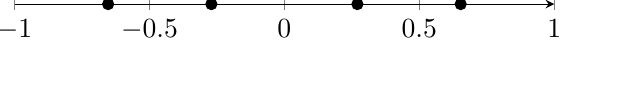
\begin{tikzpicture}
    \begin{axis}[
            axis x line=middle,
            axis y line=none,
            height=50pt,
            width=\axisdefaultwidth,
            xmin=-1,
            xmax=1,
        ]
            \addplot [only marks] coordinates {
            (0.2706,0)
            (0.6533,0)
            (-0.2706,0)
            (-0.6533,0)
            };
    \end{axis}
    \end{tikzpicture}
    \end{center}
    A naive way of clustering or partitioning these data points would be by splitting them into clusters whose components are positive and those whose components are negative. We have seen experimentally that this is a perfectly reasonable way to cluster graphs that contain two highly connected subgraphs. 

    For more chaotic graphs, or those with more than two subgraphs, this strategy will not work because there simply is not enough leeway in how we can delineate subgraphs. The idea of partitioning based on sign is still useful though, we just instead consider higher dimensional data; we extract more than one Laplacian eigenvector. In practice, which eigenvectors that are chosen are based on the nature of the graph. For simplicity, we will just consider the $N$ smallest eigenvectors.

    In the next section, we detail two algorithms that utilize these $N$-dimensional row vectors to cluster a graph.
    
\section{Algorithms}\label{sec:algo}

    For experimentation and analysis, we utilize two primary algorithms to partition our data. The first, Naive Fiedler Clustering, has been developed and written by us (see Section \ref{sec:code}). The second, k-means Clustering, is a standard data clustering method and so we employ MATLAB's implementation.

    \subsection{Naive Fiedler Clustering}

        Given some parameter $N$, which indicates how many eigenvectors to consider, we construct the matrix $X$ by treating the eigenvectors as column vectors and concatenating them horizontally,
        \[X = \left[\begin{array}{c | c | c | c } x_1 & x_2 & \cdots & x_N \end{array}\right].\]
        As stated previously, we then view the entries as $N$-dimensional row vectors.
        
        Proceeding by example, we consider the case where $N=2$ (the data here is taken directly from Experiment 1, Test 1). After constructing $X$, we apply the logical operator '$<0$' to the matrix, which for some $x_{ij} \in X$, sets $x_{ij} = 1$ if true, and $x_{ij} = 0$ if false.
        \[X = \begin{bmatrix}
            x_{11} & x_{11} \\
            x_{12} & x_{12} \\
            x_{13} & x_{13} \\
            \vdots & \vdots     
        \end{bmatrix} = \begin{bmatrix}
            \phantom{-}0.1200 & -0.0695 \\
            \phantom{-}0.0770 & -0.0793 \\
            -0.1586 & -0.1481 \\
            \phantom{-}0.0312 & \phantom{-}0.1249 \\
            \vdots & \vdots 
        \end{bmatrix} \xrightarrow{T_<} \begin{bmatrix}
            0 & 1 \\
            0 & 1 \\
            1 & 1 \\
            0 & 0 \\
            \vdots & \vdots     
        \end{bmatrix} = X_{<}\]
        This process partitions the members of $X$ based on sign, which we can use as a form of initial clustering. We can consider two vectors to be part of the same initial cluster if the result of this operator results in the same vector. For example, both $\begin{bmatrix} 0.1200 & -0.0695 \end{bmatrix}$ and $\begin{bmatrix} 0.0770 & -0.0793 \end{bmatrix}$ map to the vector $\begin{bmatrix} 0 & 1 \end{bmatrix}$ and so are clustered together. 
        
        Since there are two options for each coordinate (it is either positive or negative), we have a total of four possible image vectors: $\begin{bmatrix} 0 & 0 \end{bmatrix}$, $\begin{bmatrix} 0 & 1 \end{bmatrix}$, $\begin{bmatrix} 1 & 0 \end{bmatrix}$, $\begin{bmatrix} 1 & 1 \end{bmatrix}$. We can then construct (up to) four matrices whose members are the pre-images under each image vector. Then, the initial clustering process terminates and these matrices can be assigned a unique sub-graph. Doing this for $X_2$, which contains members whose images are all $\begin{bmatrix} 0 & 1 \end{bmatrix}$, we have
        \[X_2 = \begin{bmatrix}
            0.1200 & -0.0695 \\
            0.0770 & -0.0793 \\
            0.0936 & -0.0491 \\
            0.0303 & -0.0642 \\
            \vdots & \vdots  
        \end{bmatrix}.\]
        It is prudent to note that there is no explicit optimization process being done here (we are not minimizing an objective function). Nevertheless, it can be experimentally shown that the result of this initial clustering minimizes the cut (the number of edge connections that must be removed such that the resultant graph is disconnected) of a given graph.
        
        While this is a perfectly fine initial process, there are a few inherent flaws if we terminate here. The primary issue is that the upper bound on the number of image vectors is $2^N$, which (experimentally) tends to overshoot the number of `true' clusters present in a graph. Furthermore, the hypothetical vectors $\begin{bmatrix} -0.002 & 0.151 \end{bmatrix}$ and $\begin{bmatrix} 0.0008 & 0.152 \end{bmatrix}$ have different images, whilst in $N$-dimensional space they are quite close (see Figure \ref{fig:spatial}).
        
        \begin{figure}[h!]
            \centering
            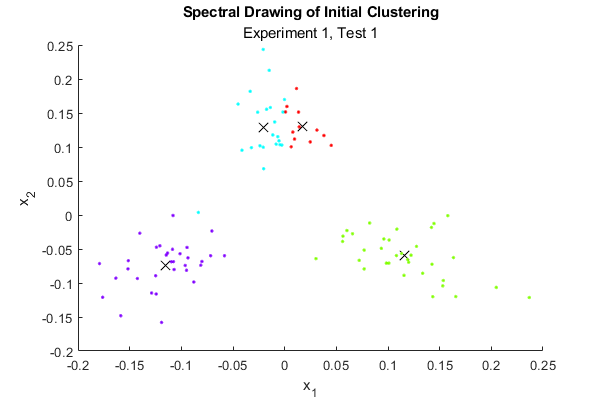
\includegraphics[width=0.75\linewidth]{images/spectral_drawing.png}
            \caption{Initial clustering based on the sign. The different color groups represent clusters, and the `x' is their centroid.}
            \label{fig:spatial}
        \end{figure}
        
        We remedy this by computing the centroids (the $N$-dimensional centre) of each cluster $X_i$. For $X_2$, we have
        \[\mu_2 = \frac{1}{n_2} \sum_{x_i \in X_2}x_i = \begin{bmatrix}
            0.1159 & -0.0601
        \end{bmatrix}\]
        
        We can then compute the Euclidean distance between centroids. Given some parameter $\varepsilon$, if $d(\mu_i, \mu_j) \leq \varepsilon$, then we consider cluster $X_i$ and $X_j$ to be sufficiently similar and thus, we can combine the clusters. Otherwise, we consider them distinct and accept the initial clustering. The clustering process then terminates, and the matrices are assigned unique subgraphs as before.
        
        Due to the complexity of the algorithm, the parameter $\varepsilon$ must be supplied before the clustering process. In other words, the optimization process is susceptible to human error. In an ideal setting, the algorithm would incorporate cohesion and/or separation (see Section \ref{sec:valid}) into an objective function, and thus automatically determine which clusters are to be combined, and which ones to be left as-is.

    \subsection{\textit{k}-means Clustering}

        For a collection of $N$-dimensional data points with $k$ desired clusters, the result of the $k$-means process is that data points are assigned to $k$ clusters in such a way that the total sum of squared errors (a form of cohesion) of the clustering is minimized. In practice, the distance function used is parameterizable and is generally based on the nature of the data in question.
        
        The $k$-means process begins by selecting $k$ initial centroids. There are several algorithms for doing this (notably `$k$-means\texttt{++}') but for the sake of simplicity, we will select them randomly. We then create $k$ initial clusters which are defined by their centroids. We compute the distance between each data point to all centroids and assign the point to the cluster whose centroid is closest (in the Euclidean sense). The centroid of each cluster is then recomputed. 
        
        The process of (1) computing distances, (2) assigning points to centroids, (3) recomputing centroids, is repeated until either the recomputed centroids are sufficiently similar (i.e. the process doesn't change) or a max number of iterations is reached. The clusters are then returned and can be used to construct subgraphs.

\section{Cluster Validation}\label{sec:valid}

    In this section, we outline two categories of metrics that quantify how `good' a given data clustering is. Internal metrics, as the name suggests, utilize information internal to the clustering process. On the other hand, external metrics are a bit more removed and involve outside information such as class labels in determining goodness. These metrics were largely obtained from \parencite[\S 23]{bennett} and \cite{cluster}.

    \subsection{Internal Metrics}

        While there are more internal metrics, the two we focus on are \emph{cohesion} and \emph{separation}.
    
        \begin{definition}
            For data cluster $X_i$ with centroid $\mu_i$, the \emph{cohesion} of cluster $X_i$ is defined as
            \[\text{cohesion}(X_i) = \sum_{x_j \in X_i} d(x_j, \mu_i)\]
            where $d$ is any distance function. The cohesion of a clustering $X$, with clusters $X_1, X_2, \ldots, X_n$ and centroids $\mu_1, \mu_2, \ldots, \mu_n$, is defined as 
            \[\text{cohesion}(X) = \sum_{X_i \in X} \sum_{x_j \in X_i} d(x_j, \mu_i)\]
        \end{definition}
    
        As stated prior, the cohesion of the clustering (with Euclidean distance) is the objective function being minimized by $k$-means.
        
        \begin{definition}
            For data clusters $X_i, X_j$ with centroids $\mu_i, \mu_j$, the \emph{separation} between clusters $X_i, X_j$ is defined as
            \[\text{separation}(X_i, X_j) = d(\mu_i, \mu_j)\]
            where $d$ is any distance function. The separation of a clustering $X$, with clusters $X_1, X_2, \ldots, X_n$ and centroids $\mu_1, \mu_2, \ldots, \mu_n$, is defined as 
            \[\text{separation}(X) = \sum_{X_i \in X} w_i \cdot d(\mu_i, \mu^*)\]
            where $w$ is a set of weights, and $\mu^*$ is the centroid of $X$ (the centroid of the data set).
        \end{definition}
    
        While not explicitly employed, one can consider naive Fiedler to be implicitly maximizing separation as a byproduct of the cluster combination step; if clusters are too close (i.e. separation is too small), then we combine clusters and thus increase separation.

    \subsection{External Metrics}

        The first external metric, \emph{accuracy}, requires that the correct clustering be known beforehand. Further, the number of computed clusters must be the same as the number of correct clusters. The second clustering metric, \emph{agreement}, just requires that the number of computed clusters between clusterings be equal.
        
        \begin{definition}
            Given a known correct clustering $X^*$, the \emph{accuracy} of a computed clustering $X$ is simply the ratio between correctly classified objects and the total number of objects. An accuracy close to 1 indicates better clustering. 
            
            Given two computed clusterings $X, X^\prime$ if one of them is treated as the `correct' clustering, then the accuracy metric becomes an \emph{agreement} metric. An agreement close to 1 indicates a strong similarity between clusterings.
        \end{definition}
    
        For our experiments, we have constructed the graphs ourselves so the true clusterings are known prior (hence, accuracy is usable). In practice, this is generally not the case and so accuracy is an unusable metric. The following two metrics are far more flexible in that all that needs to be supplied is some set of labels $C$, whose count does not need to match the number of clusters.
    
        \begin{definition}
            Given a clustering $X = \{X_1, \ldots, X_n\}$, and some set of labels $C = \{C_1, \ldots, C_m\}$, we can define the \emph{entropy} of cluster $X_i$ to be
            \[\text{entropy}(X_i) = (-1)\cdot \sum_{C_i \in C} P(x_{C_i}) \log_2(P(x_{C_i}))\]
            where $P(x_{C_i})$ is the probability that $x \in X_i$ belongs to label $C_i \in C$. If this probability is unknown, then we can substitute this probability for the \emph{maximum likelihood estimate} (MSE) of this probability
            \[\text{entropy}(X_i) = (-1)\cdot \sum_{C_i \in C} \frac{|x_{C_i}|}{n_{X_i}} \log_2\left(\frac{|x_{C_i}|}{n_{X_i}}\right)\]
            where $|x_{C_i}|$ is the number of objects classified as label $C_i$ in cluster $X_i$, and $n_{X_i}$ is the number of objects in cluster $X_i$.
            
            We can then define the total entropy of a clustering as
            \[\text{entropy}(X) = \sum_{X_i \in X} \frac{n_{X_i}}{n} \cdot \text{entropy}(X_i)\]
            where $n_{X_i}$ is the number of objects in cluster $X_i$, and $n$ is the total number of objects in the clustering $X$. An entropy closer to $0$ indicates a better clustering and an entropy closer to $1$ indicates a worse clustering.
        \end{definition}
    
        To better elucidate this rather technical definition, the entropy of a clustering can be thought of as the `spread' of the computed clustering relative to the cluster labels. As another aid, we will showcase the entropy calculation for Experiment 1, Test 2. Constructing the confusion matrix (which is a diagrammatic way of interpreting the clustering), we have
    
        \begin{center}
        {\makegapedcells
        \begin{tabular}{cc|cccc}
        \multicolumn{2}{c}{}
            & \multicolumn{3}{c}{Actual} \\
            & & $C_1$ & $C_2$ & $C_3$ \\ 
            \cline{2-5}
        \multirow{2}{*}{\rotatebox[origin=c]{90}{Calc.}}
            & $X_1$ & 34 &  1 & 33 \\
            & $X_2$ &  0 & 32 &  0 \\ 
            \cline{2-5}
        \end{tabular}}
        \captionof{table}{Confusion matrix for Experiment 1, Test 2}
        \end{center}
        We can then compute the entropy by reading off of the table
        \[\text{entropy}(X_1) = (-1)\cdot\left( \frac{34}{68}\log_2\left(\frac{34}{68}\right) + \frac{1}{68}\log_2\left(\frac{1}{68}\right) + \frac{33}{68}\log_2\left(\frac{33}{68}\right) \right) = 1.0957\]
        \[\text{entropy}(X_2) = (-1)\cdot\left( \frac{32}{32}\log_2\left(\frac{32}{32}\right) \right) = 0\]
        The total entropy is then
        \[\text{entropy}(X) = \frac{68}{100}(1.0957) + \frac{32}{100}(0) = 0.7451\]
        This corroborates our intuition that it is a worse clustering than Test 1 (see Section \ref{sec:exp}).
        
        \begin{definition}
            Given a clustering $X = \{X_1, \ldots, X_n\}$, and some set of labels $C = \{C_1, \ldots, C_m\}$, we can define the \emph{purity} of cluster $X_i$ to be
            \[\text{purity}(X_i) = \max_{C_i \in C} P(x_{C_i}) \text{ or } \max_{C_i \in C} \frac{|x_{C_i}|}{n_{X_i}}\]
            where $P(x_{C_i})$ is the probability that $x \in X_i$ belongs to label $C_i \in C$, and $|x_{C_i}| / n_{X_i}$ is the MSE, as stated prior.
    
            The purity of the clustering $X$ is then defined as
            \[\text{purity}(X) = \sum_{X_i \in X} \frac{n_{X_i}}{n} \cdot \text{purity}(X_i)\]
            A purity closer to $1$ indicates better clustering, and a purity closer to $0$ indicates worse clustering.
        \end{definition}
    
        In using metrics to quantify the goodness of a clustering, it is pivotal that multiple be used. For example, a high purity value (which indicates a good clustering) can be achieved when the number of clusters is large. It may be the case though that when this is contrasted with accuracy, agreement, or entropy, the clustering is quite poor!

\section{Experiments and Analysis}\label{sec:exp}

    In this section, we detail one experiment (more were done, but we ran out of space). While the graph being analyzed was constructed by hand, the specifics of the process will not be elaborated upon here. Instead, please see Section \ref{sec:code} and the file \texttt{connectedGraph.m}.

\subsection{Experiment 1}

    We construct the graph $G$ with 100 vertices and 3 inherent clusters of equal size. We set the probability that a cluster has inter-cluster edge connections as 0.75, and the probability of intra-cluster edge connections as 0.25. 

    The components of the first four eigenvectors (excluding the trivial eigenvector), which are sorted according to the first eigenvector, can be seen in Figure 2 below.

    \begin{figure}[h!]
        \centering
        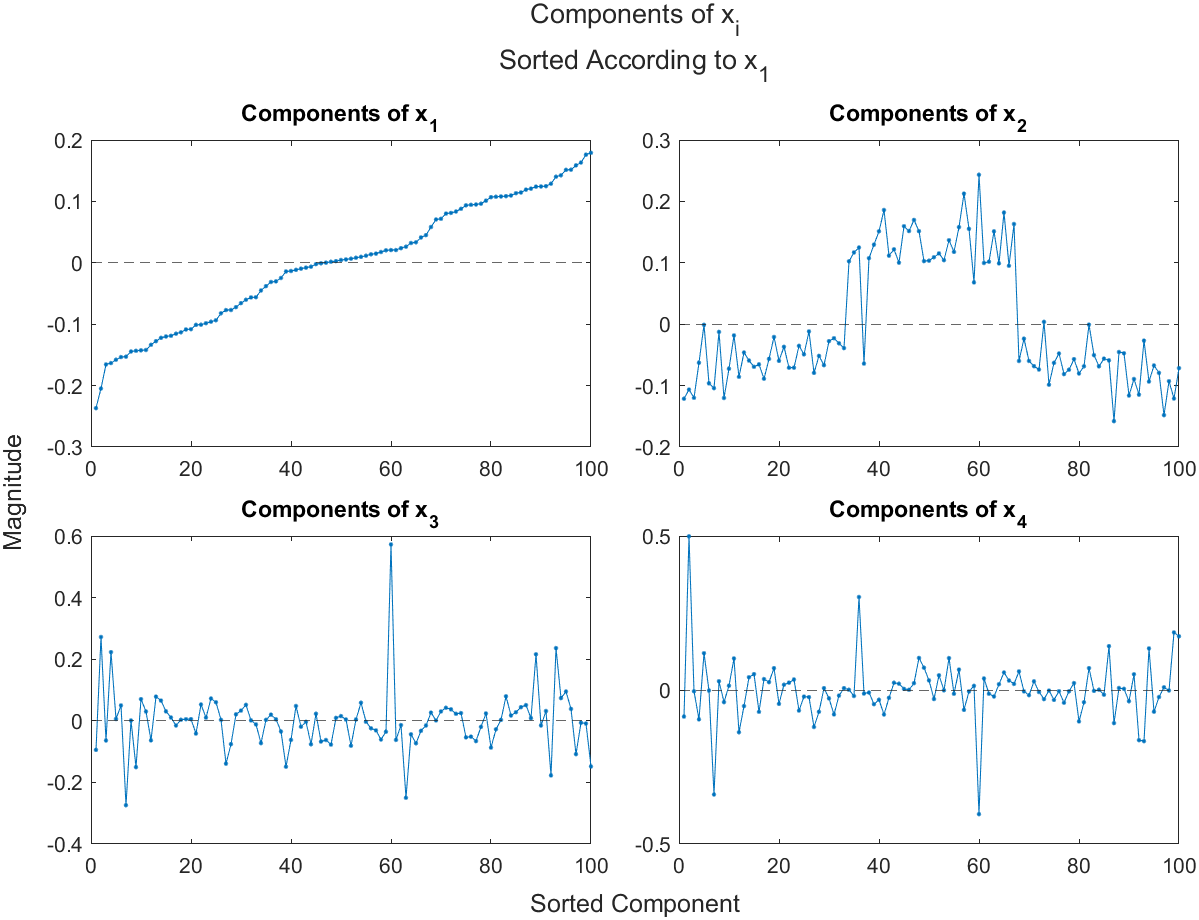
\includegraphics[width=0.75\linewidth]{images/comp.png}
        \captionof{figure}{Components of the first four eigenvectors of the graph Laplacian}
    \end{figure}

    Examining the components of the first eigenvector, though somewhat subtle, there do appear to be three visible groups present. The three groups are very visible in the components of the second eigenvector, though there does not appear to be much information contained within the components of the third and fourth eigenvectors. 
    
    Intuitively then, one might consider clustering based on the first and second eigenvectors only, ignoring the others. This is validated experimentally, and we will see that including the third and fourth eigenvectors in fact results in a worse clustering.
    
    We run two different iterations of \texttt{naiveFiedler} and \texttt{kmeansFiedler} on $G$. The first naive Fiedler test (Figure 3) examines the first two eigenvectors of the graph Laplacian, while the second (Figure 4) examines the first four. Both have a tolerance $\varepsilon$ of 0.20. Both $k$-means are computed with $k=3$, though the first test (Figure 5) examines the first eigenvector whereas the second (Figure 6) examines the first and second eigenvectors.

    \begin{figure}[h!]
        \centering
        \begin{minipage}{.35\textwidth}
          \centering
          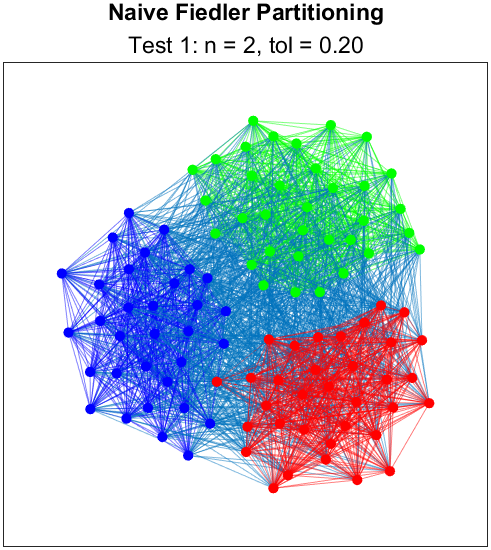
\includegraphics[width=0.95\linewidth]{images/naive1.png}
          \captionof{figure}{}
        \end{minipage}%
        \begin{minipage}{.35\textwidth}
          \centering
          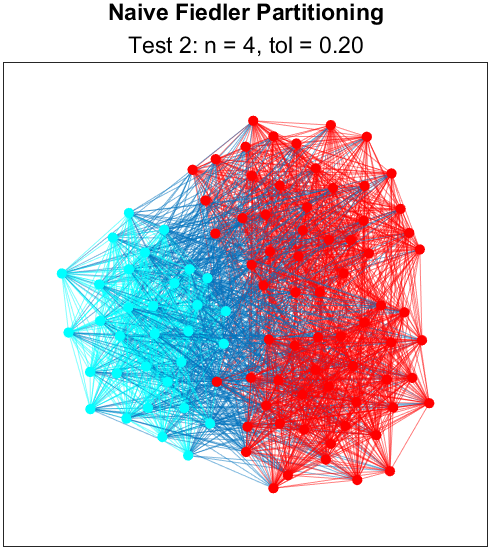
\includegraphics[width=0.95\linewidth]{images/naive2.png}
          \captionof{figure}{}
        \end{minipage}
    \end{figure}

    \begin{figure}[h!]
        \centering
        \begin{minipage}{.35\textwidth}
          \centering
          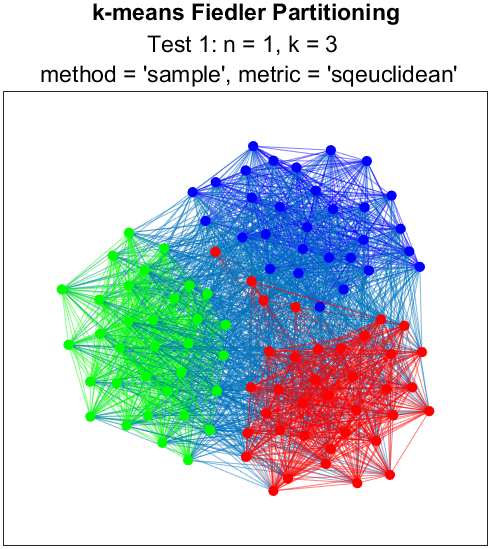
\includegraphics[width=0.95\linewidth]{images/kmeans1.png}
          \captionof{figure}{}
        \end{minipage}%
        \begin{minipage}{.35\textwidth}
          \centering
          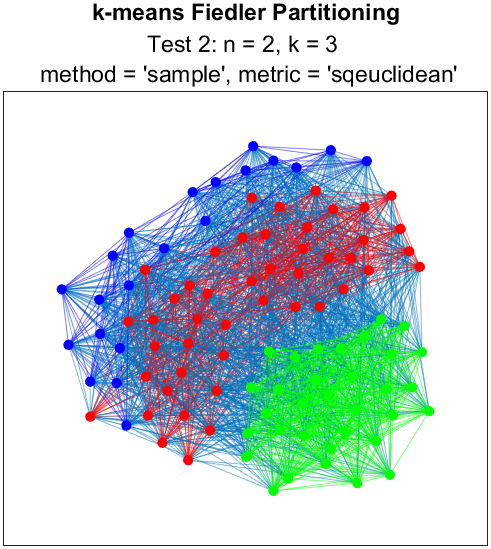
\includegraphics[width=0.95\linewidth]{images/kmeans2.png}
          \captionof{figure}{}
        \end{minipage}
    \end{figure}

    Inspecting the figures visually, we see that naive Fiedler (test 1), and $k$-means (test 1) perform quite similarly. This is corroborated by an agreement value of 0.95 (see Table 2(b)). Viewing Table 2(a), we see that naive Fiedler (test 1) is the superior clustering in all of accuracy, entropy, and purity. For both algorithms, we see that the presence of more data (more eigenvectors) results in a worse clustering visually as well as numerically. 

    \begin{table}[h!]%\[!htb\]
    \centering
    \caption{Cluster validity measures}
    \begin{subtable}[t]{.4\textwidth}
        \caption{Individual cluster metrics}
        \raggedright
        \begin{tabular}{|c|c|c|c|} \hline
                              & Accuracy & Entropy & Purity \\ \hline
            $\text{Naive}_1$  &   0.9900 &  0.0651 & 0.9900 \\ \hline
            $\text{Naive}_2$  &        - &  0.7451 & 0.6600 \\ \hline
            $\text{kmeans}_1$ &   0.9600 &  0.1828 & 0.9600 \\ \hline
            $\text{kmeans}_2$ &   0.7000 &  0.6644 & 0.7000 \\ \hline
        \end{tabular}
    \end{subtable}%
    \begin{subtable}[t]{.55\textwidth}
        \raggedleft
        \caption{Agreement between clusterings}
        \begin{tabular}{|c|c|c|c|c|} \hline
                              & $\text{Naive}_1$ & $\text{Naive}_2$ & $\text{kmeans}_1$ & $\text{kmeans}_2$ \\ \hline
            $\text{Naive}_1$  &                - &                - &            0.9500 &            0.7000 \\ \hline
            $\text{Naive}_2$  &                - &                - &                 - &                 - \\ \hline
            $\text{kmeans}_1$ &           0.9500 &                - &                 - &            0.6600 \\ \hline
            $\text{kmeans}_2$ &           0.7000 &                - &            0.6600 &                 - \\ \hline
        \end{tabular}
    \end{subtable}
    \end{table}

\section{Closing Remarks}\label{sec:conc}

    Spectral clustering utilizes concepts from spectral graph theory and linear algebra to separate, or in this case, cluster, graphs to identify similar groups of nodes as well as anomalies. We have demonstrated these properties by applying naive Fiedler and k-means clustering methods on generated data. Depending on the desired results, both clustering methods are valid ways of analyzing data.
    
    While an elegant technique, the results obtained via spectral clustering are solely dependent on the algorithm being used. Computational complexity aside, the $k$-means algorithm must be presented with an appropriate initial $k$-value and initial centroid parameters. Otherwise, the algorithm runs the risk of ``getting stuck'' in a local minimum and producing inaccurate clusters. Additionally, numerous outliers may warp the final shape of the clusters, as it increases the total sum of squared errors. Care must be taken to implement several different internal and external validity metrics to ensure the accuracy of the final product. 
    
    One possible objective function to implement is something called the `Dunn Index' which incorporates both cohesion and separation and is to be maximized. Given further time, we could conceivably write our own $k$-means method that utilizes this. Concerning naive Fiedler clustering, there is no explicit objective function - which is highly problematic. As stated previously, this would be remedied by introducing cohesion (or separation) to be minimized (or maximized) in the second step.

    In this paper, we have been primarily concerned with connected graphs that are unweighted. The obvious follow-up is to consider disconnected and weighted graphs. Further, we have been constructing the graphs to be experimented upon. Investigating spectral clustering algorithms on real-world data would be far more enlightening and interesting.

\section{Code}\label{sec:code}

    Please see \url{https://github.com/agormann/MATH-309} for all the code used.

\printbibliography

\end{document}
